\documentclass{article}
\usepackage[margin=1in]{geometry}
\usepackage[utf8]{inputenc}
\usepackage{graphicx} 
\usepackage{fancyhdr}
\usepackage{enumitem}
\usepackage{lipsum}
\usepackage[bahasa]{babel}
\usepackage{subcaption}
\usepackage{float}
\usepackage{indentfirst}

\title{Laporan Workshop Telematika \\ Dasar Desain Schematic dan PCB} % Ganti sesuai modul praktikum yang diikuti
\author{Azaria Putri Fawnia \\ 5024221038} % Ganti dengan NRP dan Nama Kalian

\date{}


\fancypagestyle{firstpageheader}{
  \fancyhf{} 
  \fancyhead[L]{
\includegraphics[height=1.5cm]{img/logodepart.png}} 
  \fancyhead[R]{Institut Teknologi Sepuluh Nopember \\ Departemen Teknik Komputer \\ Laboratorium Robotika dan Sistem Cerdas} 
  \renewcommand{\headrulewidth}{0pt} 
  \fancyfoot[C]{%
    
\includegraphics[width=\textwidth]{img/footer.png}
  }
  \renewcommand{\footrulewidth}{0pt} % No line in the footer
}


\fancyhf{} 
\fancyfoot[C]{%
  
\includegraphics[width=\textwidth]{img/footer.png}
}
\renewcommand{\headrulewidth}{0pt} 
\renewcommand{\footrulewidth}{0pt} 

\pagestyle{fancy}
\begin{document}
\selectlanguage{bahasa}
\maketitle
\thispagestyle{firstpageheader}
% Bagian Tugas Pendahuluan
\section*{Tugas Pendahuluan}
\begin{enumerate}
  \item Install Fusion 360 pada Laptop masing-masing anggota kelompok \\
  \begin{figure}[H]
    \centering
    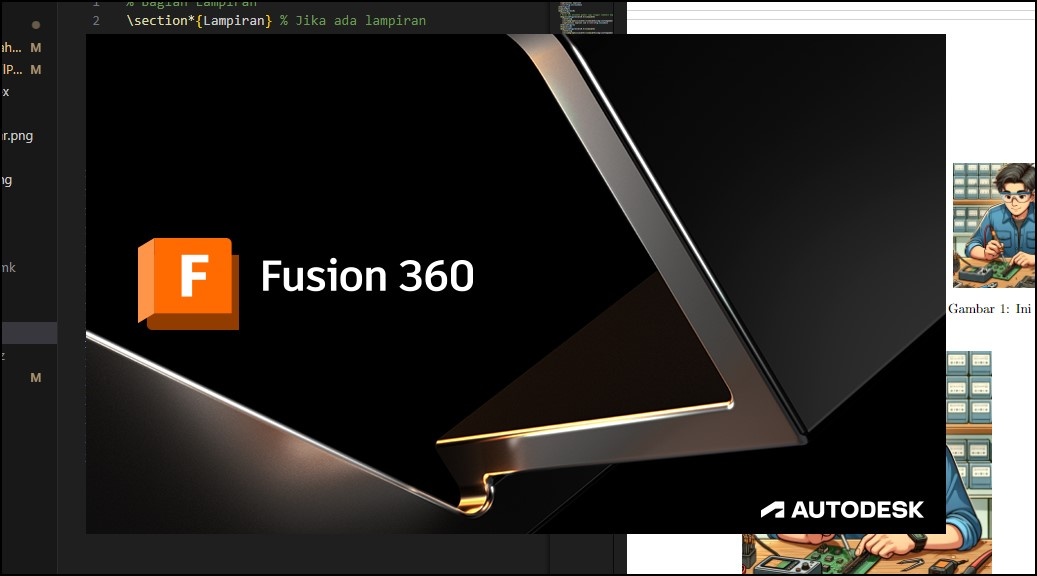
\includegraphics[width=0.6\linewidth]{img/buktidownloadfusion360.jpg}
    \caption{Bukti install FUSION 360} 
  \end{figure}
  \item Buat jalur PCB rangkaian regulator lm7805 dari schematic yang telah disediakan
  pada folder praktikan \\
  \begin{figure}[H]
    \centering
    % Kalau mau menambah gambar lagi tinggal nambahin begin{subfigure} -> end{subfigure}
    \begin{subfigure}[b]{0.45\linewidth}
      \centering
      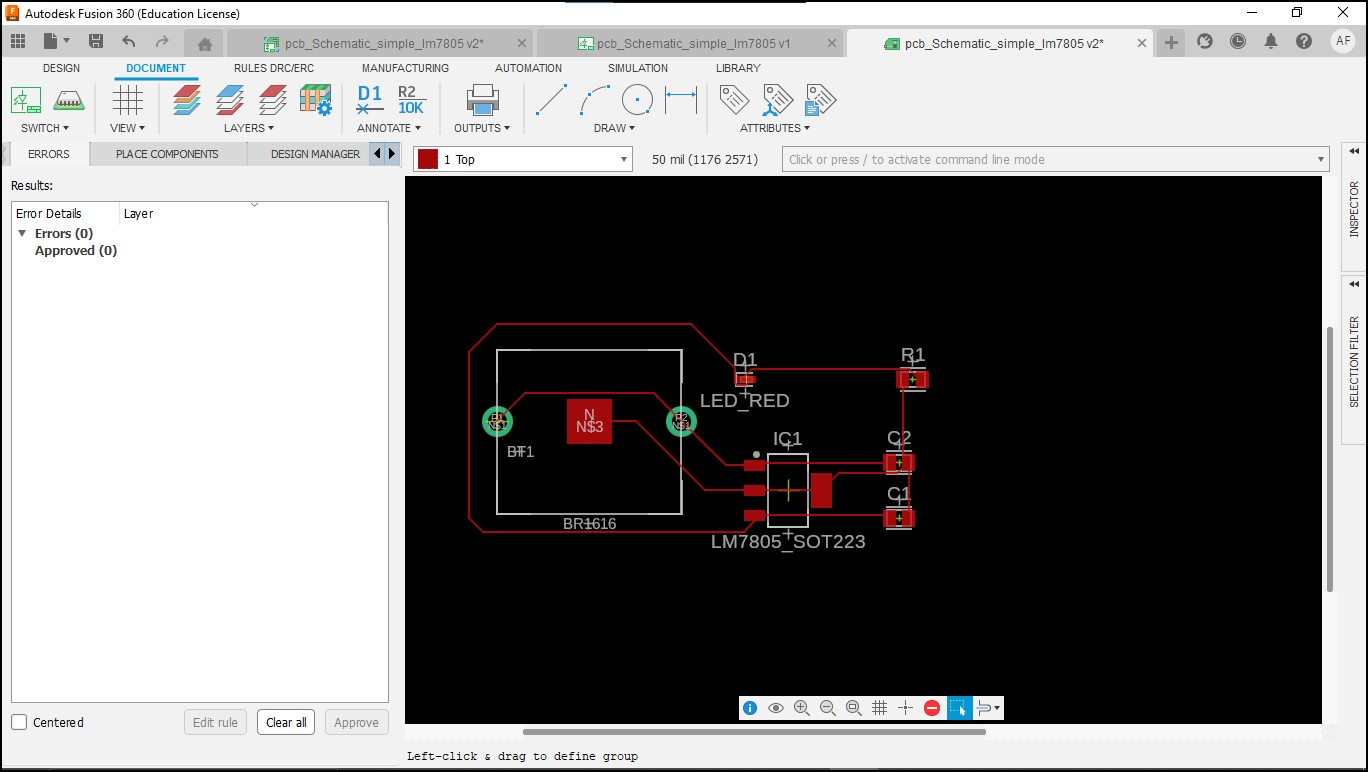
\includegraphics[width=\linewidth]{img/buatpcb.jpg}
      \caption{Bukti desain PCB\label{fig:inisub1}}
    \end{subfigure}
    \hspace{1cm}
    \begin{subfigure}[b]{0.45\linewidth}
      \centering
      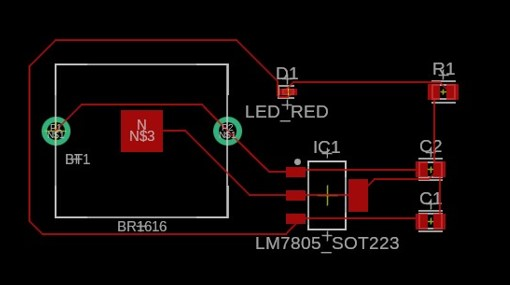
\includegraphics[width=\linewidth]{img/buatpcb(2).jpg}
      \caption{Jalur PCB\label{fig:inisub2}}
    \end{subfigure}
    \caption{Membuat jalur PCB rangkaian regulator lm7805 dari schematic yang telah disediakan\label{fig:keduagambar}}
  \end{figure}
\end{enumerate}
% Bagian Analisis Hasil Percobaan
\section*{Analisis Hasil Percobaan}
\indent
Pada gambar \ref{fig:inirujukan} dapat dilihat bahwa pada tabel \ref{tab:labelini} terdapat data yang menunjukkan bahwa \lipsum[1]
\lipsum[1-2]

\begin{table}[h]
    \centering
    \caption{Caption tabelnya}
    \label{tab:labelini}
    \begin{tabular}{|c|c|c|c|}
    \hline
    Kolom 1 & Kolom 2 & Kolom 3 & Kolom 4 \\
    \hline
    Data 1 & Data 2 & Data 3 & coba nambah kolom \\
    Data 4 & Data 5 & Data 6 & coba nambah kolom juga \\ 
    \hline
    \end{tabular}
\end{table}
% Bagian Lampiran
\section*{Lampiran} % Jika ada lampiran
\begin{figure}[H]
  \centering
  
\includegraphics[width=0.2\linewidth]{img/contohgambar.png}
  \caption{Ini Caption} 
  \label{fig:inirujukan}
\end{figure}
\vspace{0pt}
\begin{figure}[H]
  \centering
  % Kalau mau menambah gambar lagi tinggal nambahin begin{subfigure} -> end{subfigure}
  \begin{subfigure}[b]{0.4\linewidth}
    \centering
    
\includegraphics[width=\linewidth]{img/contohgambar.png}
    \caption{Ini Caption sub 1\label{fig:inisub1}}
  \end{subfigure}
  \hspace{1cm}
  \begin{subfigure}[b]{0.4\linewidth}
    \centering
    
\includegraphics[width=\linewidth]{img/contohgambar.png}
    \caption{Ini Caption sub 2\label{fig:inisub2}}
  \end{subfigure}
  \caption{Caption kedua gambar\label{fig:keduagambar}}
\end{figure}
\end{document}